\apendice{Documentación de usuario}

\section{Introducción}
Debido a que el desarrollo se enfocó en la realización del backend, me enfrenté al desafío de identificar cómo podrían hacer los miembros del tribunal evaluador para probar las APIs desarrolladas tanto del backend como del chatbot, no existiendo aún la aplicación como tal.
Para ello me desafié a buscar una solución que permitiera ejecutarse en la nube de forma que no fuera necesario instalar un software en cada computadora para las pruebas.

\section{Requisitos de usuarios}
Como herramienta de pruebas para los usuarios se ha seleccionado Postman Web ya que sólo con contar con un navegador web es suficiente para este software.

A continuación, se detallan los requisitos mínimos para poder ejecutarse las pruebas, en base al navegador del que se disponga.

\begin{itemize}
\tightlist
\item
  \texttt{Chrome}: versión 78 o superior.
  \item
  \texttt{Firefox}: versión 76 o superior.
  \item
  \texttt{Edge}: versión 79 o superior.
  \item
  \texttt{Safari}: versión 13.1.1 o superior.
\end{itemize}

\section{Manual del usuario}

\subsection{Backend}

Para poder realizar las pruebas los usuarios deberán de navegar a la siguiente url: \href{https://www.postman.com/cloudy-space-109868/workspace/emur/collection/27053529-4afae92f-7a66-4091-ad9b-50f499e2d515}{Postman Web}.\\
Allí encontrarán las colecciones de endpoints creadas para el backend y chatbot de la futura aplicación móvil de EM (ver figura~\ref{Img:Coleccion+Postman+Usuario}).
\begin{figure}[h]
    \centering
    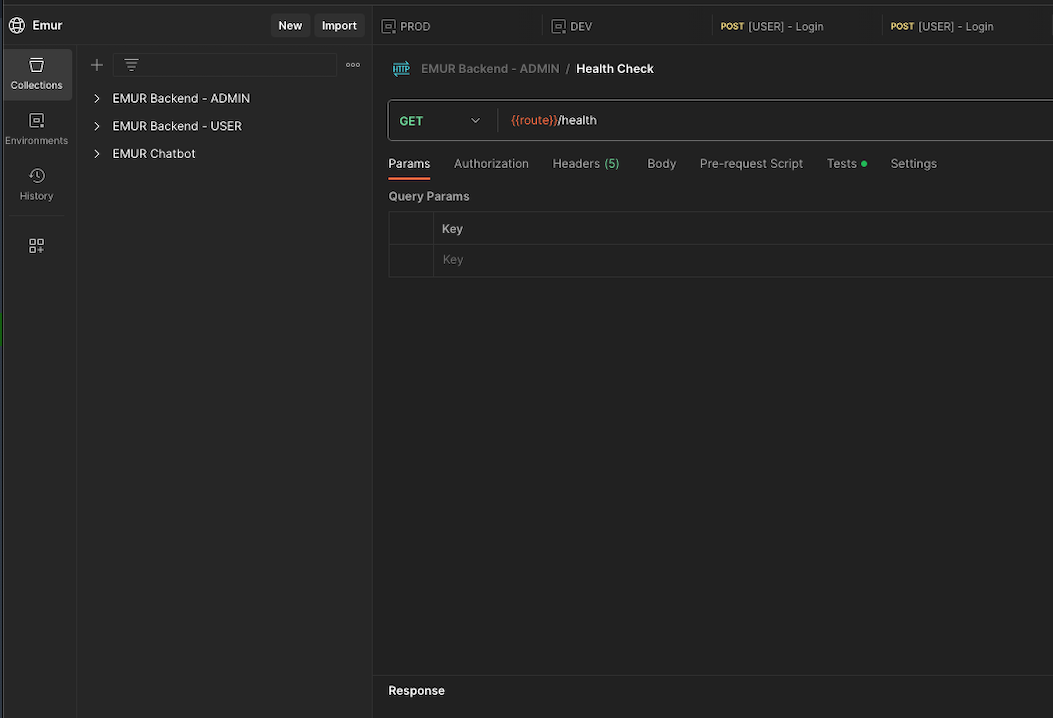
\includegraphics[width=1.1\textwidth]{img/usuario/colecciones_postman1.png}
    \caption{Colección de APIs de Backend y Chatbot} \label{Img:Coleccion+Postman+Usuario}
\end{figure} 

Una vez allí, las colecciones se muestran colapsadas, para tal fin debemos hacer clic sobre la colección que queremos abrir. En el caso del presente proyecto, existen 3 colecciones debido a que una es para probar con rol administrador, otra es con el rol de usuario y la tercera para probar el chatbot (ver figura~\ref{Img:Coleccion+Postman+Usuario+2}).

\newpage
\begin{figure}[h]
    \centering
    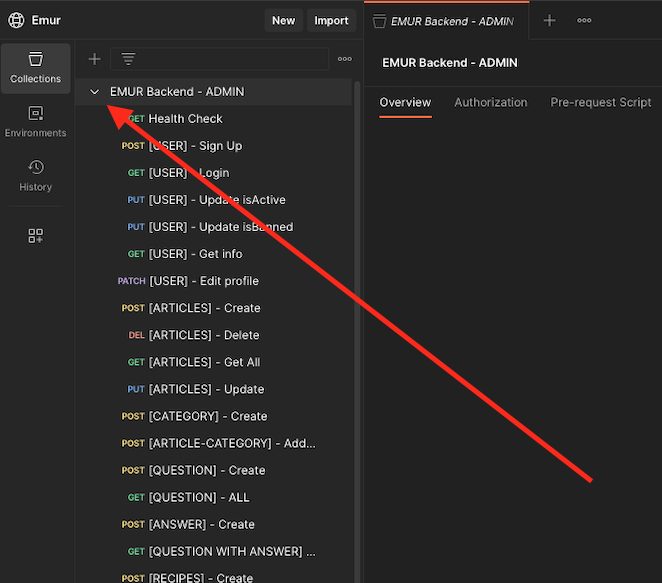
\includegraphics[width=0.8\textwidth]{img/usuario/colecciones_postman2.png}
    \caption{Cómo abrir las colecciones} \label{Img:Coleccion+Postman+Usuario+2}
\end{figure} 

Una vez tenemos la colección abierta podemos proceder a probar los endpoints. A continuación se explica cómo hacerlo.

\begin{itemize}
\tightlist
\item
  \texttt{Paso 1}: Clic en el menú izquierdo sobre [QUESTION] - CREATE
  \item
  \texttt{Paso 2}: Nos dirigimos a Body.
  \item
  \texttt{Paso 3}: En el apartado 3, remplazamos el contenido a la key llamada text con el texto que se desee.
  \item
  \texttt{Paso  4}: Presionamos sobre Send.
    \item
  \texttt{Paso  5}: Observamos el resultado del operación ejecutada.
\end{itemize}

Con los puntos anteriores podemos fácilmente manejar la creación de request hacía la API para acceder a las diferentes operaciones que tendrá la futura aplicación móvil.
A modo de mejor entendimiento, se disponibiliza un video en el siguiente enlace:
\href{https://www.dropbox.com/s/3b3uwcgpcwrhlkx/grabacion_question_answer.mov?dl=0}{Video en Dropbox}

A modo de facilitar las pruebas, los endpoints en Postman cuentan con datos precargados.

\subsection{Chatbot}

Para el caso del chatbot, las pruebas se realizan de la misma forma, se ha disponibilizado bajo una colección llamada Chatbot, donde se puede acceder al endpoint para realizar las preguntas que se deseen.

También, a modo de tutorial, se ha disponibilizado un video en el siguiente enlace:
\href{https://www.dropbox.com/s/hgilnzncrb17aju/chatbot.mov?dl=0}{Video en Dropbox}





